\chapter{Normal Burst Histograms}
\label{app:hists}

\par In Figures \ref{fig:app_hist_phib}--\ref{fig:app_hist_ap}, we present histograms showing the distributions of $\phi_B$, $a_B$, $\sigma_B$, $c$, $\phi_d$, $a_d$, $d$, $\lambda$, $\phi_p$ and $a_p$ we find in our population study of bursts in the Bursting Pulsar.  Each of these is a parameter we used to fit the Normal Bursts in our sample: see Section \ref{sec:struc} for a full explanation of these parameters.  In Figures \ref{fig:app_hist_phib_n}--\ref{fig:app_hist_ap_n} we show the distributions of $\phi_B$, $a_B$, $\phi_d$, $a_d$, $\phi_p$ and $a_p$ after being normalised by the persistent emission rate $k$ at the time of each burst.

\begin{figure}
  \centering
  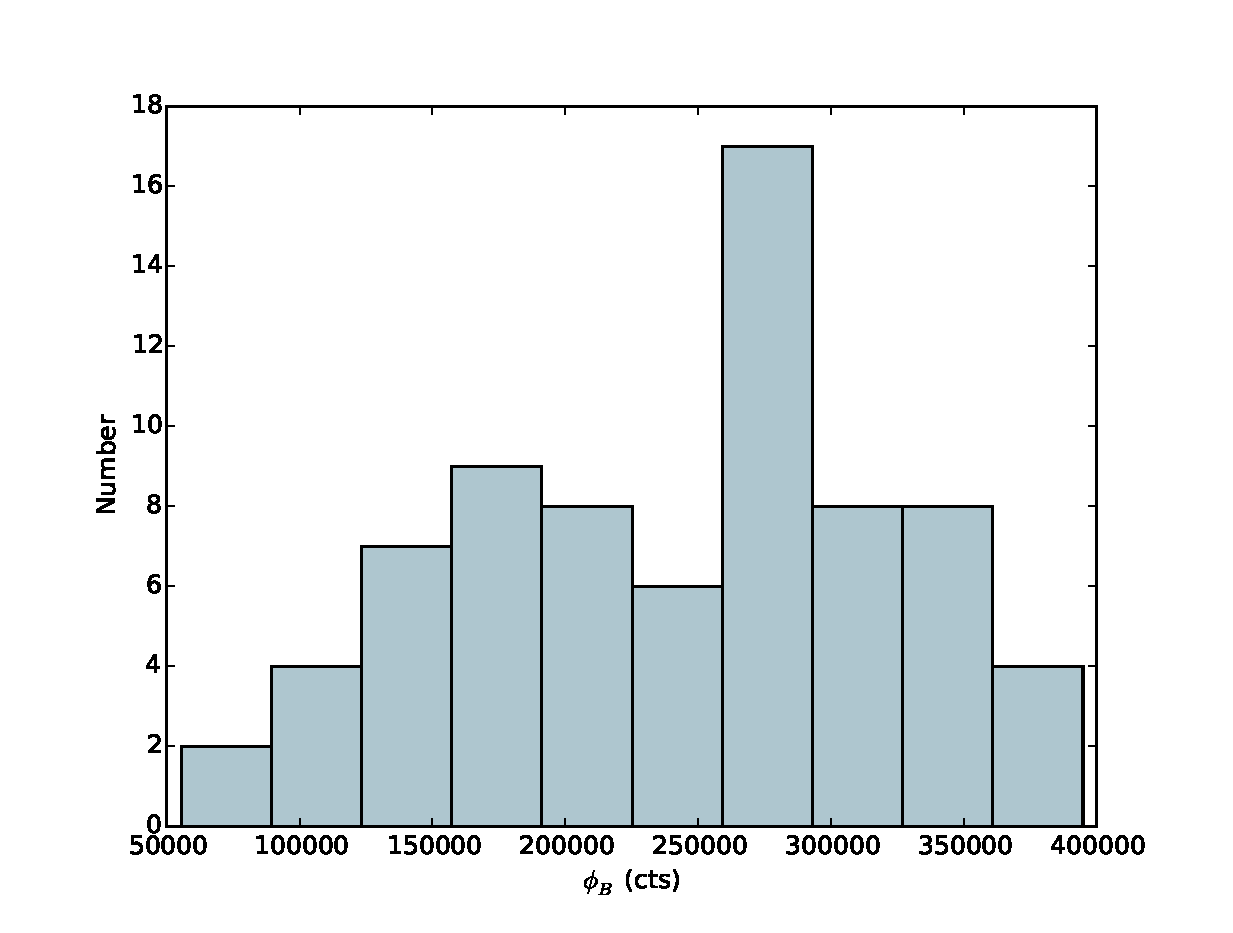
\includegraphics[width=.9\linewidth, trim={0cm 0 0cm 0},clip]{images/appendix_burst_aafluence_hist.eps}
  \caption[Histogram showing the distribution of $\phi_B$ amongst Normal Bursts.]{A histogram showing the distribution of burst fluence $\phi_B$ amongst our sample of Normal Bursts.}
  \label{fig:app_hist_phib}
\end{figure}

\begin{figure}
  \centering
  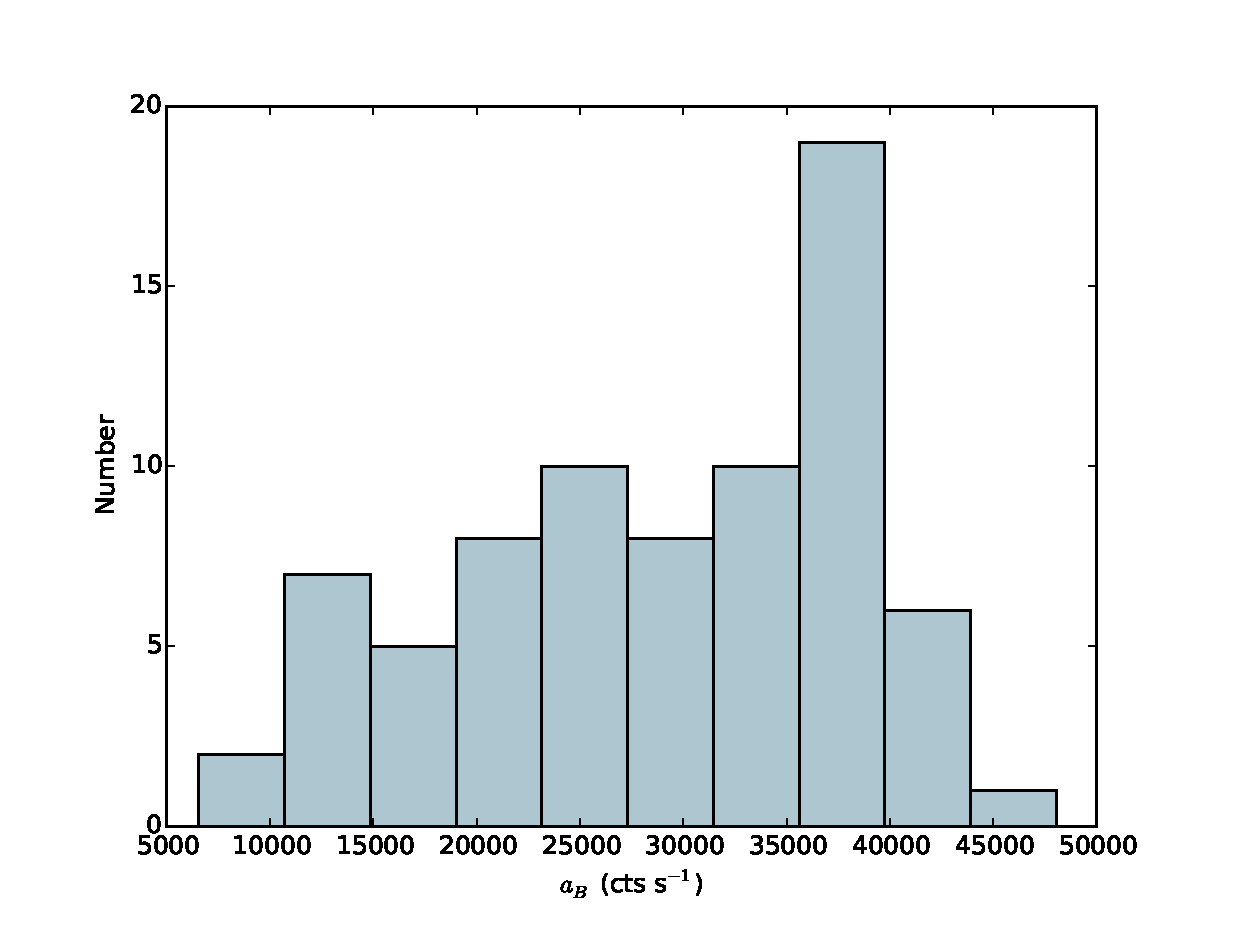
\includegraphics[width=.9\linewidth, trim={0cm 0 0cm 0},clip]{images/appendix_burst_pa_hist.eps}
  \caption[Histogram showing the distribution of $a_B$ amongst Normal Bursts.]{A histogram showing the distribution of burst amplitude $a_B$ amongst our sample of Normal Bursts.}
  \label{fig:app_hist_ab}
\end{figure}

\begin{figure}
  \centering
  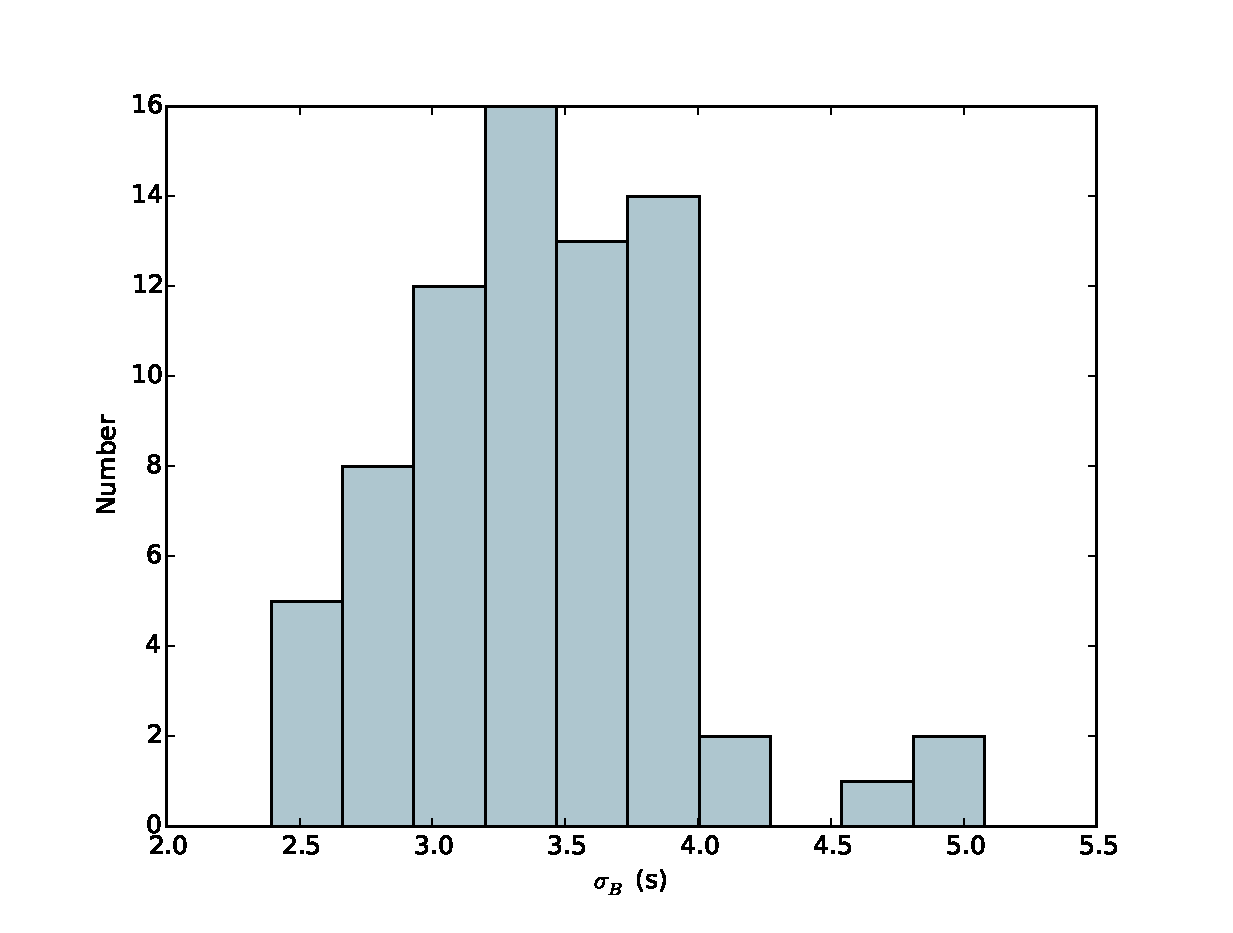
\includegraphics[width=.9\linewidth, trim={0cm 0 0cm 0},clip]{images/appendix_burst_sigma_hist.eps}
  \caption[Histogram showing the distribution of $\sigma_B$ amongst Normal Bursts.]{A histogram showing the distribution of burst width $\sigma_B$ amongst our sample of Normal Bursts.}
  \label{fig:app_hist_sigb}
\end{figure}

\begin{figure}
  \centering
  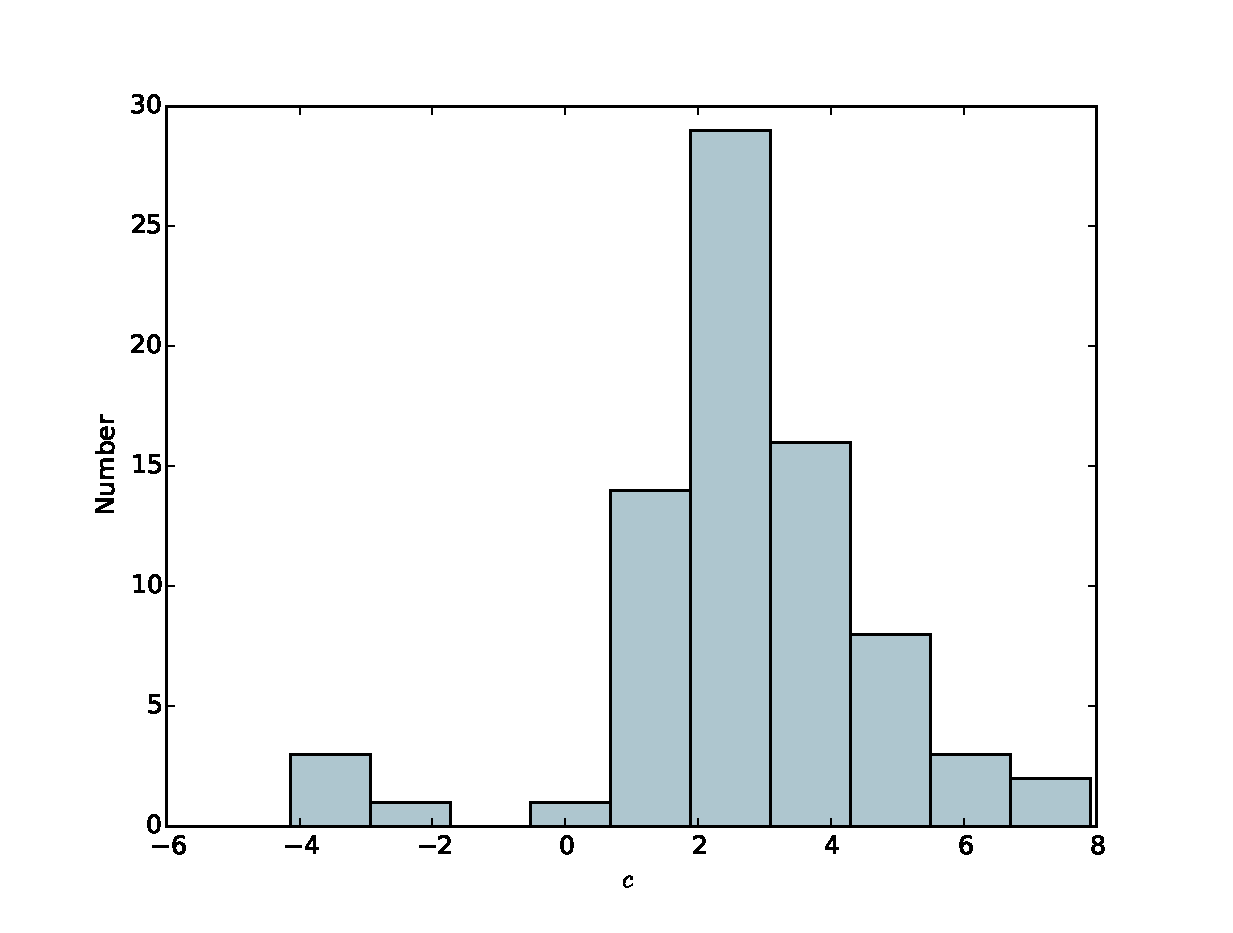
\includegraphics[width=.9\linewidth, trim={0cm 0 0cm 0},clip]{images/appendix_burst_skew_hist.eps}
  \caption[Histogram showing the distribution of $c$ amongst Normal Bursts.]{A histogram showing the distribution of burst skewness $c$ amongst our sample of Normal Bursts. }
  \label{fig:app_hist_c}
\end{figure}

\begin{figure}
  \centering
  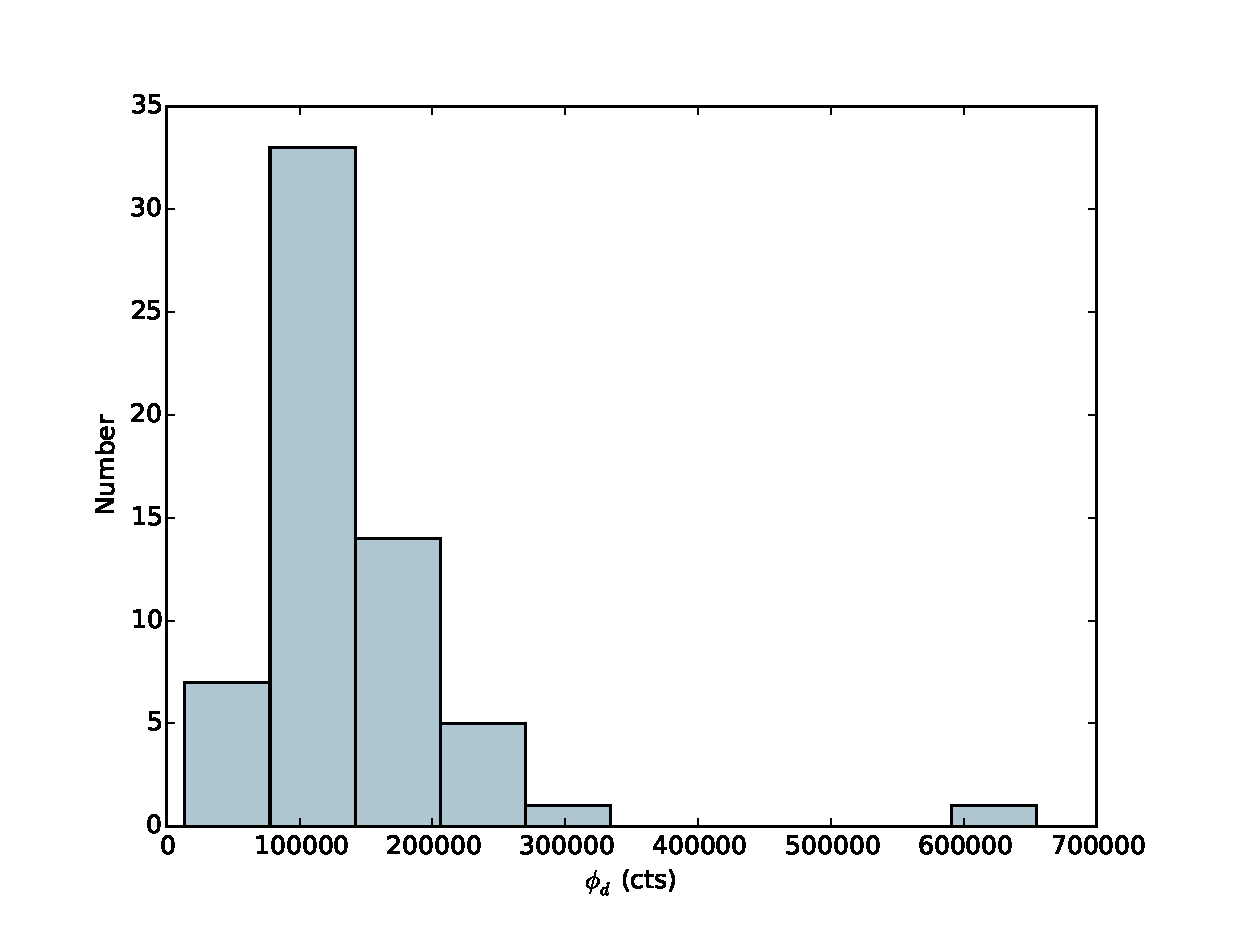
\includegraphics[width=.9\linewidth, trim={0cm 0 0cm 0},clip]{images/appendix_dip_aafluence_hist.eps}
  \caption[Histogram showing the distribution of $\phi_d$ amongst Normal Bursts.]{A histogram showing the distribution of dip fluence $\phi_d$ amongst our sample of Normal Bursts.}
  \label{fig:app_hist_phid}
\end{figure}

\begin{figure}
  \centering
  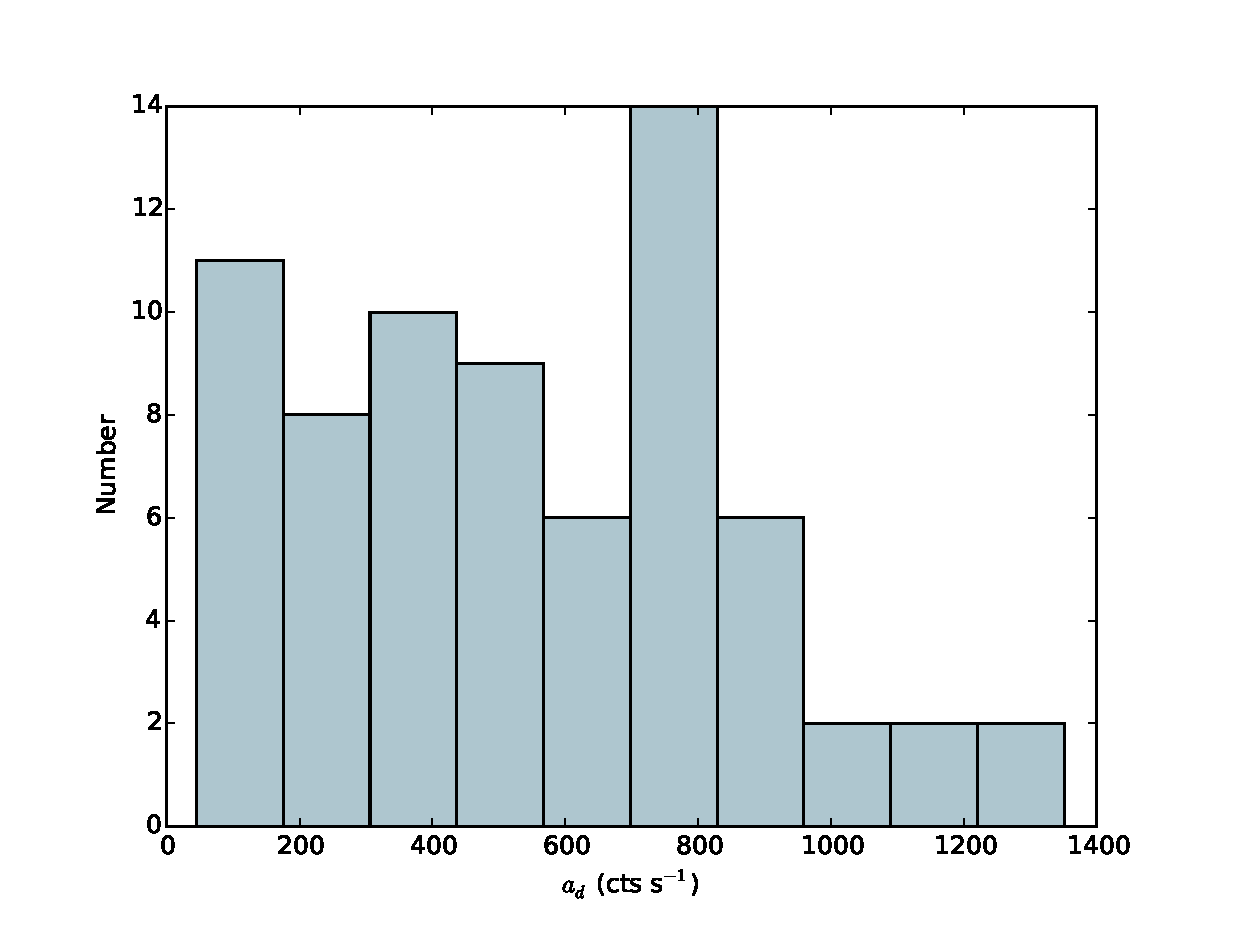
\includegraphics[width=.9\linewidth, trim={0cm 0 0cm 0},clip]{images/appendix_dip_pa_hist.eps}
  \caption[Histogram showing the distribution of $a_d$ amongst Normal Bursts.]{A histogram showing the distribution of dip amplitude $a_d$ amongst our sample of Normal Bursts.}
  \label{fig:app_hist_ad}
\end{figure}

\begin{figure}
  \centering
  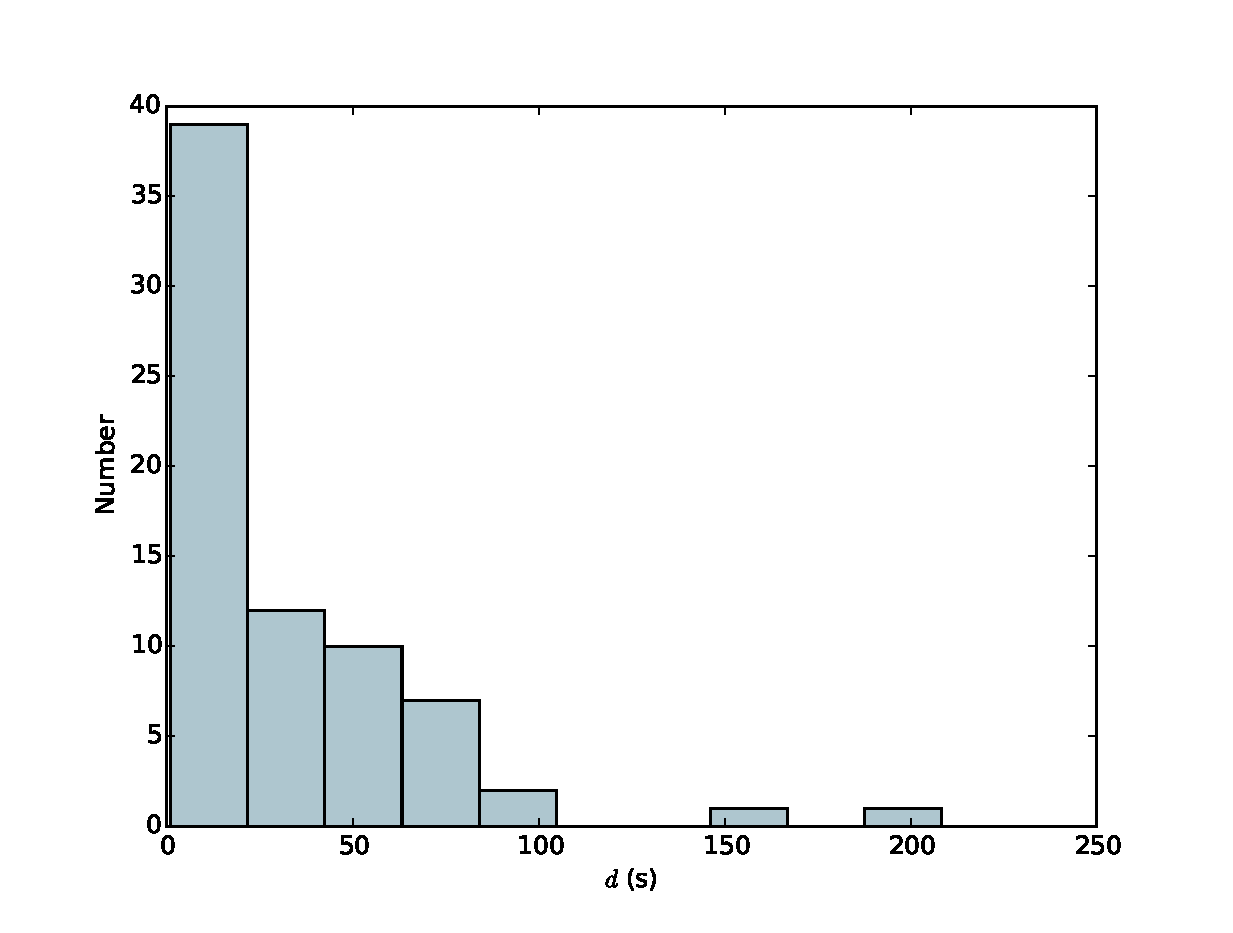
\includegraphics[width=.9\linewidth, trim={0cm 0 0cm 0},clip]{images/appendix_div_hist.eps}
  \caption[Histogram showing the distribution of $d$ amongst Normal Bursts.]{A histogram showing the distribution of dip fall-time $d$ amongst our sample of Normal Bursts.}
  \label{fig:app_hist_d}
\end{figure}

\begin{figure}
  \centering
  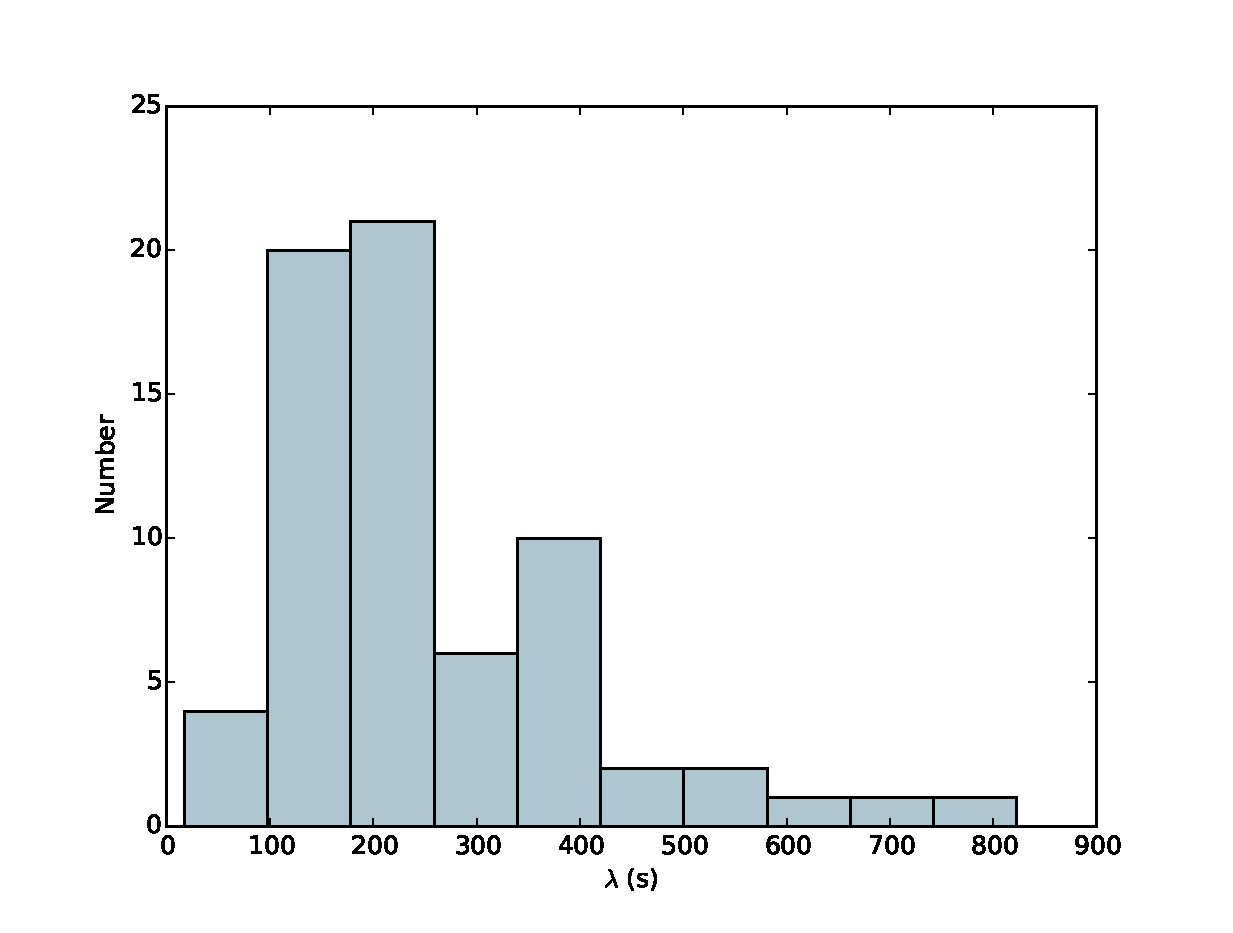
\includegraphics[width=.9\linewidth, trim={0cm 0 0cm 0},clip]{images/appendix_lambda_hist.eps}
  \caption[Histogram showing the distribution of $\lambda$ amongst Normal Bursts.]{A histogram showing the distribution of dip recovery timescale $\lambda$ amongst our sample of Normal Bursts.}
  \label{fig:app_hist_lamb}
\end{figure}

\begin{figure}
  \centering
  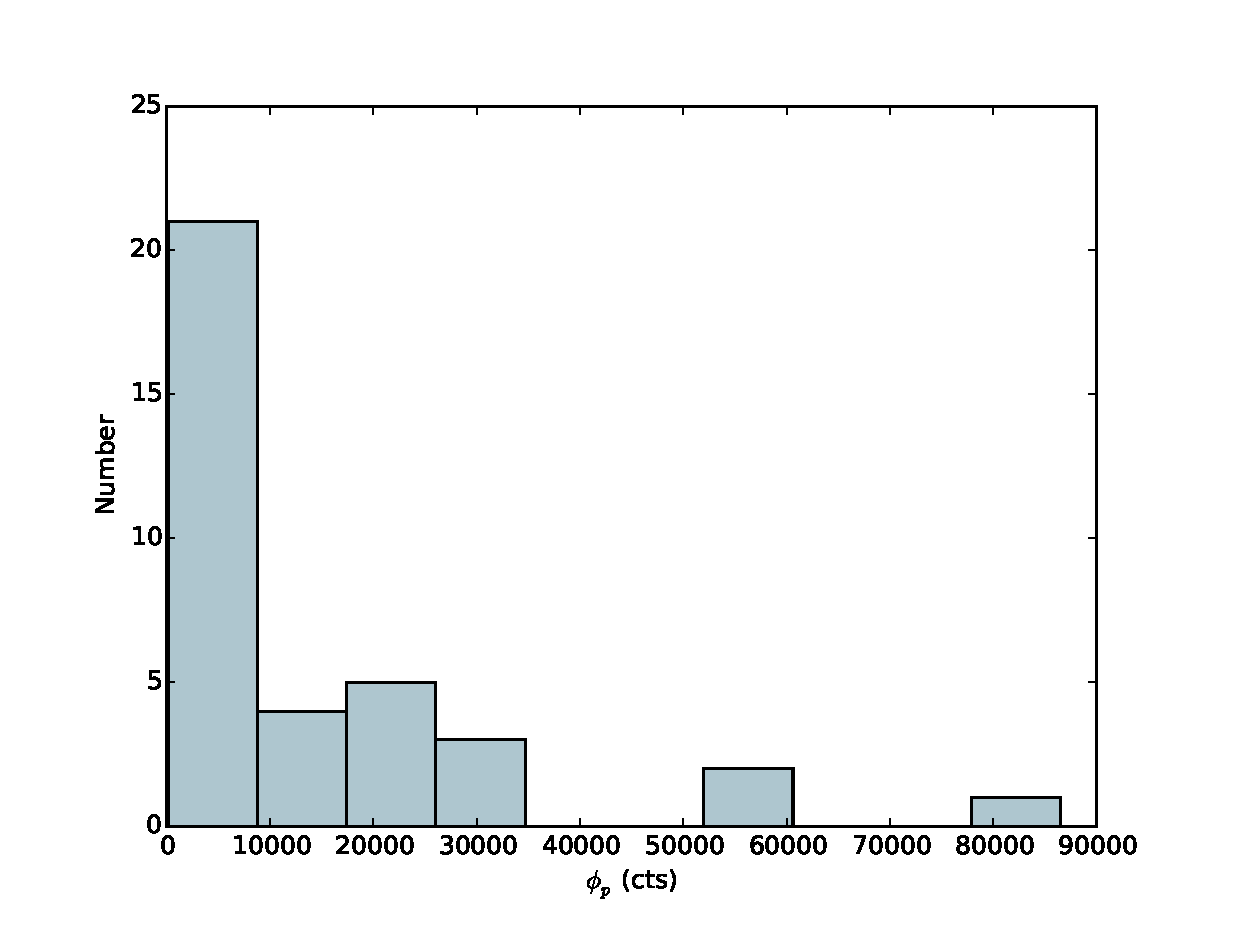
\includegraphics[width=.9\linewidth, trim={0cm 0 0cm 0},clip]{images/appendix_plat_aafluence_hist.eps}
  \caption[Histogram showing the distribution of $\phi_p$ amongst Normal Bursts.]{A histogram showing the distribution of plateau fluence $\phi_p$ amongst our sample of Normal Bursts.}
  \label{fig:app_hist_phip}
\end{figure}

\begin{figure}
  \centering
  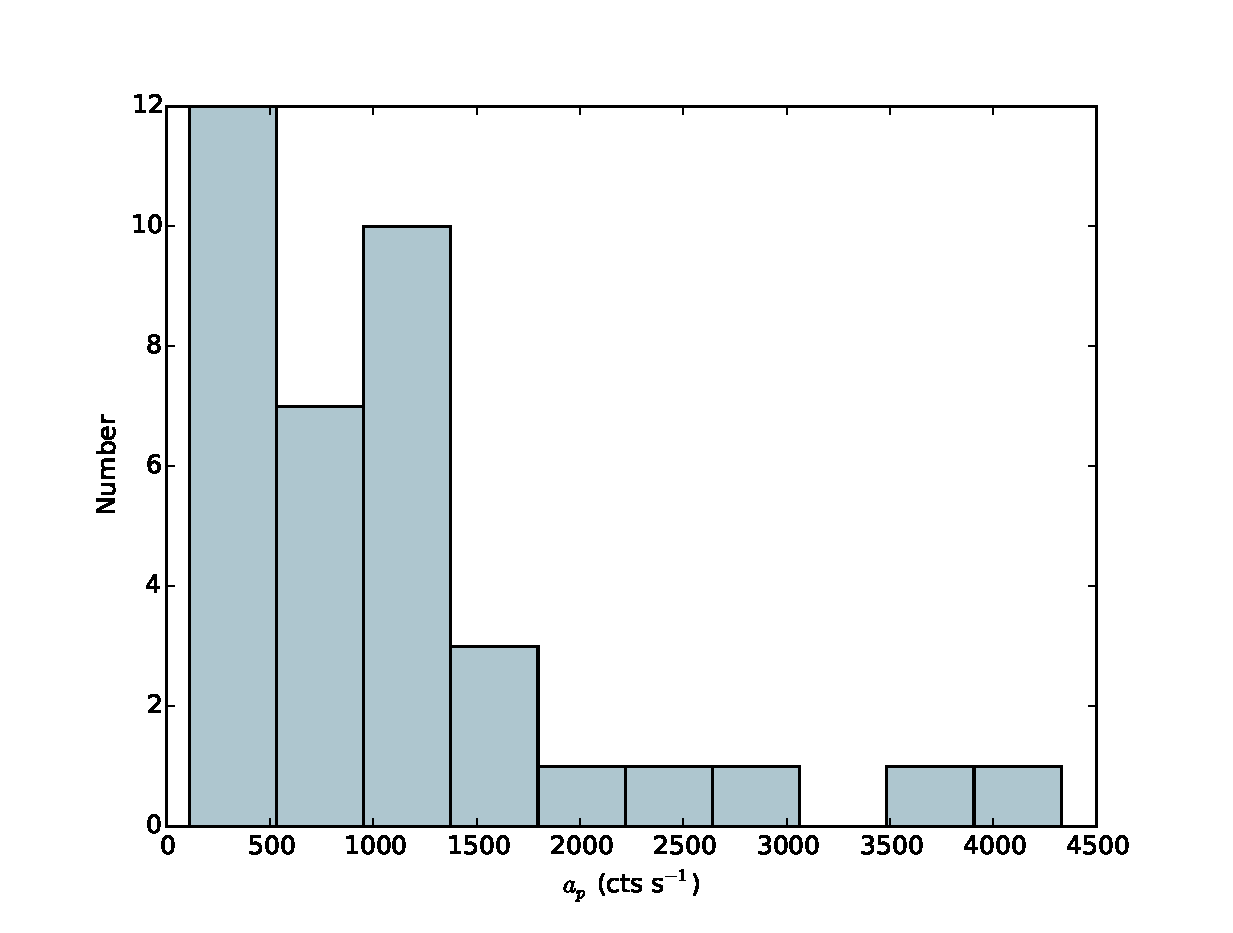
\includegraphics[width=.9\linewidth, trim={0cm 0 0cm 0},clip]{images/appendix_plat_pa_hist.eps}
  \caption[Histogram showing the distribution of $a_p$ amongst Normal Bursts.]{A histogram showing the distribution of plateau amplitude $a_p$ amongst our sample of Normal Bursts.}
  \label{fig:app_hist_ap}
\end{figure}

%-----------------

\begin{figure}
  \centering
  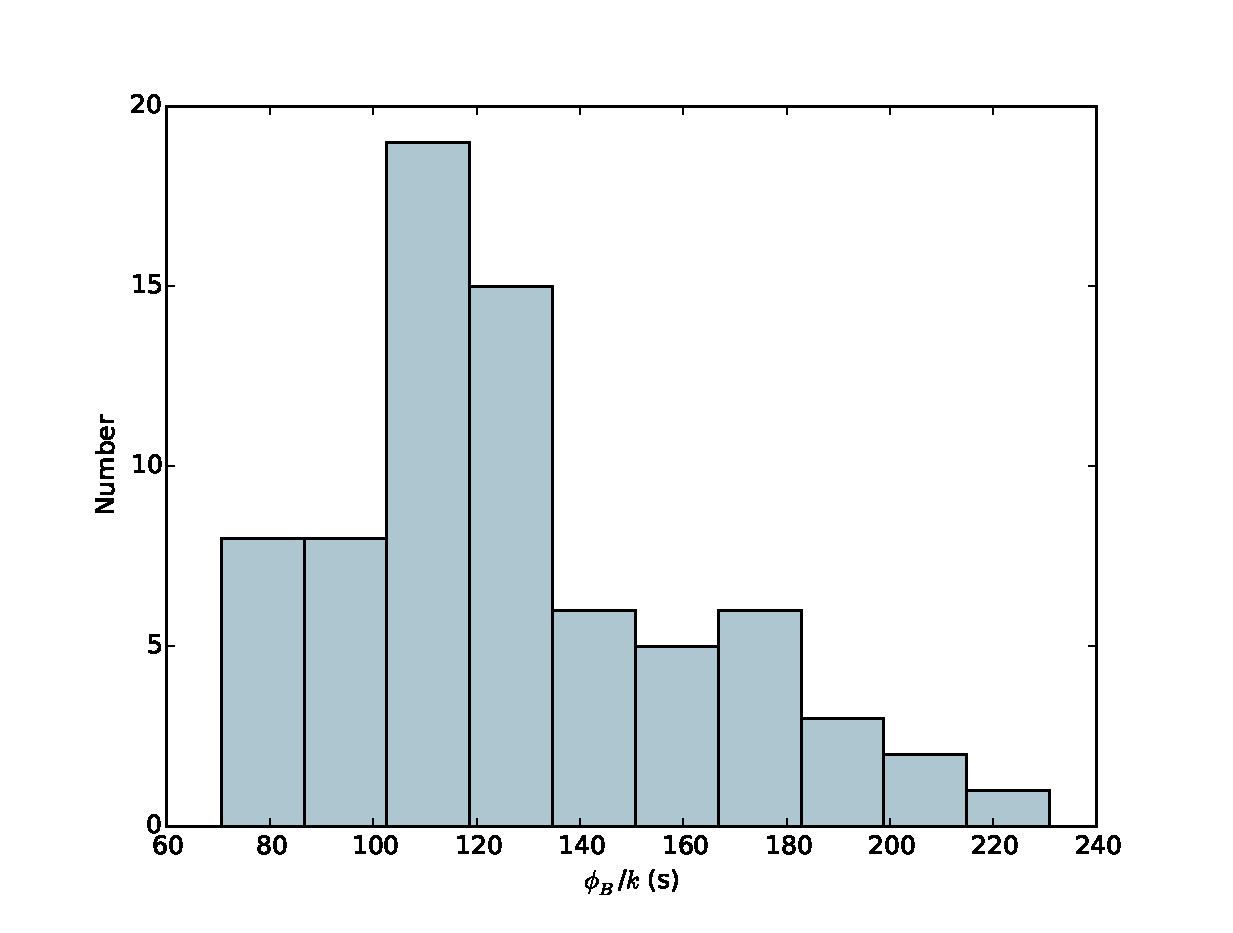
\includegraphics[width=.9\linewidth, trim={0cm 0 0cm 0},clip]{images/appendix_burst_aafluence_n_hist.eps}
  \caption[Histogram showing the distribution of $\phi_B/k$ amongst Normal Bursts.]{A histogram showing the distribution of persistent-emission-normalised burst fluence $\phi_B/k$ amongst our sample of Normal Bursts.}
  \label{fig:app_hist_phib_n}
\end{figure}

\begin{figure}
  \centering
  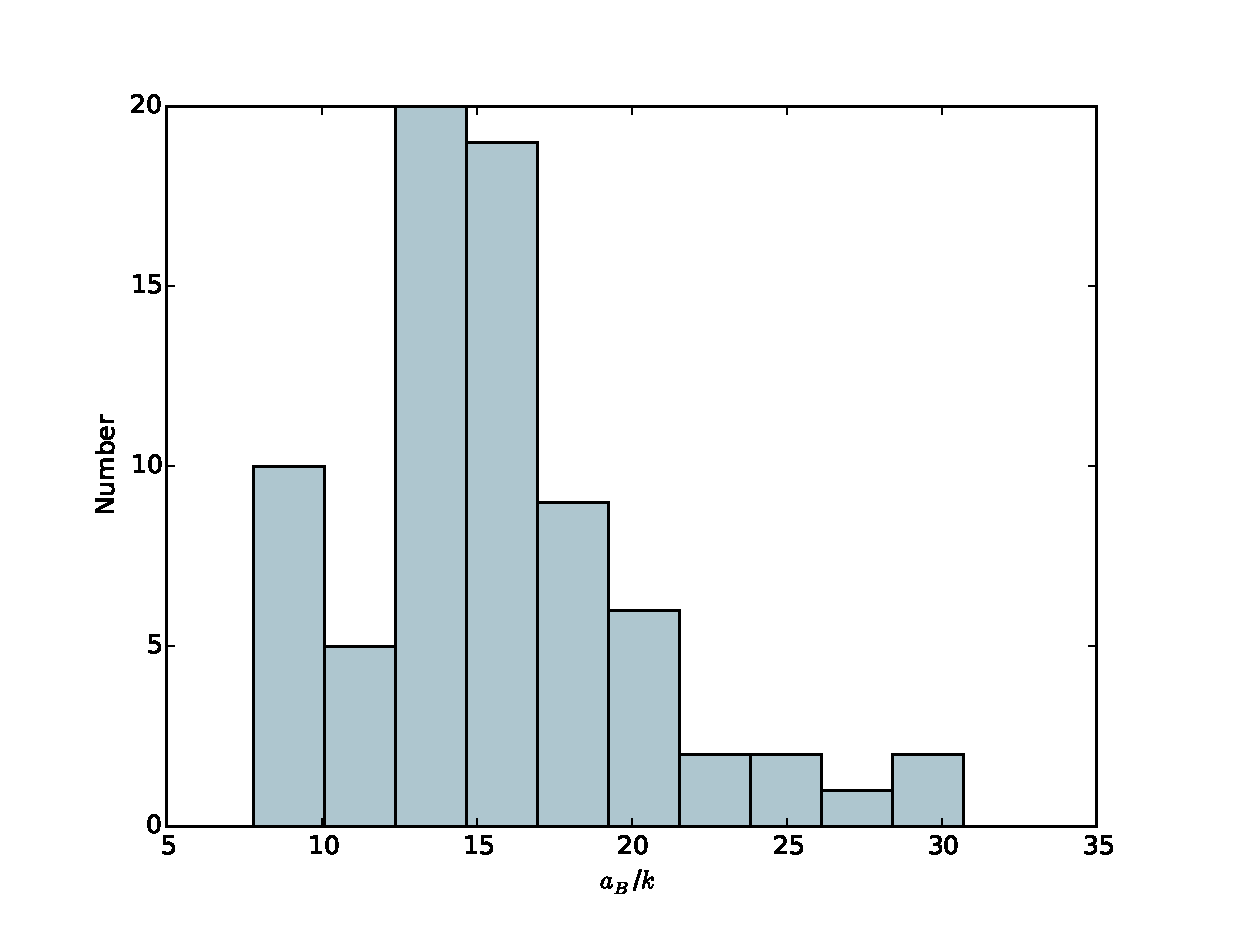
\includegraphics[width=.9\linewidth, trim={0cm 0 0cm 0},clip]{images/appendix_burst_pa_n_hist.eps}
  \caption[Histogram showing the distribution of $a_B/k$ amongst Normal Bursts.]{A histogram showing the distribution of persistent-emission-normalised burst amplitude $a_B/k$ amongst our sample of Normal Bursts.}
  \label{fig:app_hist_ab_n}
\end{figure}

\begin{figure}
  \centering
  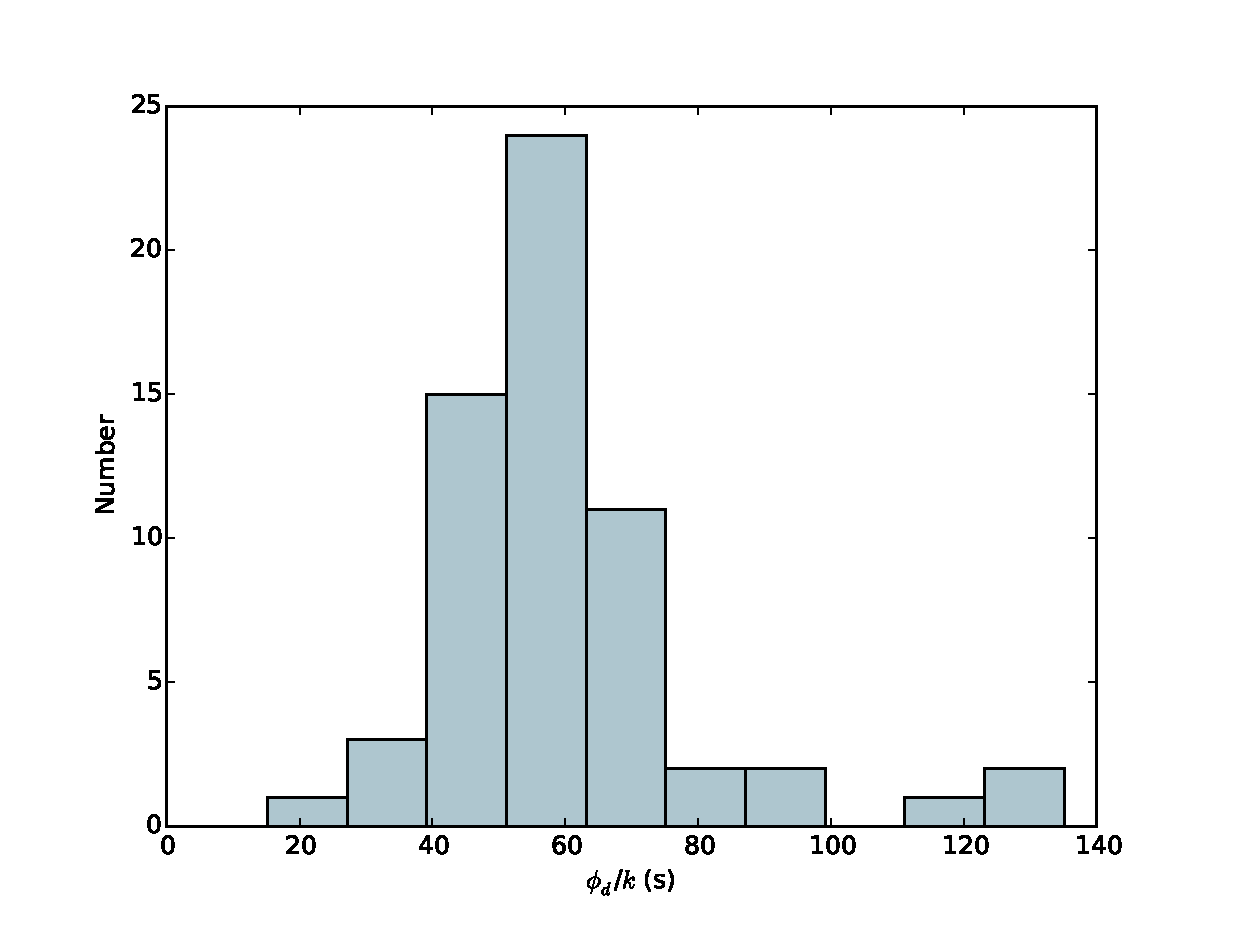
\includegraphics[width=.9\linewidth, trim={0cm 0 0cm 0},clip]{images/appendix_dip_aafluence_n_hist.eps}
  \caption[Histogram showing the distribution of $\phi_d/k$ amongst Normal Bursts.]{A histogram showing the distribution of persistent-emission-normalised dip fluence $\phi_d/k$ amongst our sample of Normal Bursts.}
  \label{fig:app_hist_phid_n}
\end{figure}

\begin{figure}
  \centering
  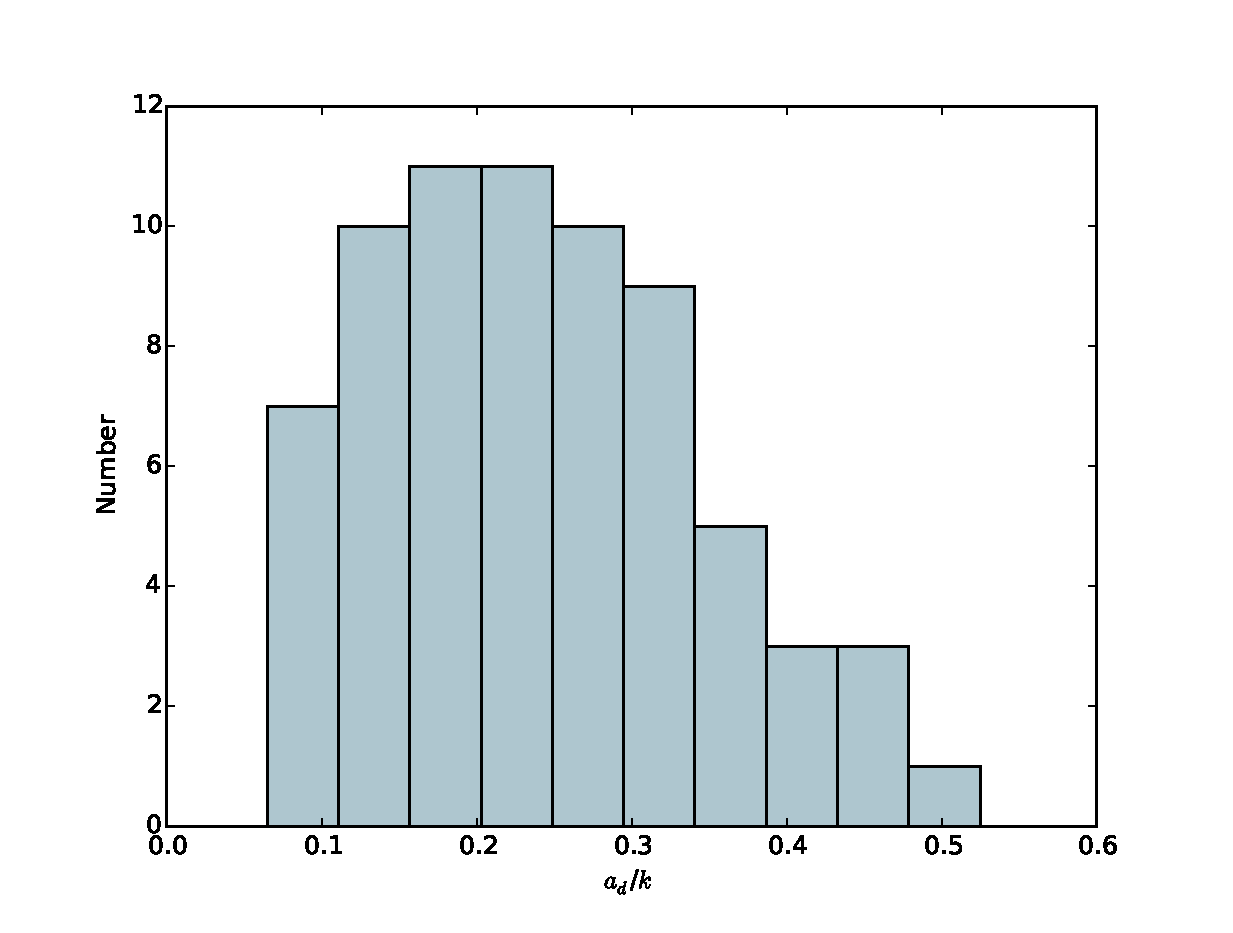
\includegraphics[width=.9\linewidth, trim={0cm 0 0cm 0},clip]{images/appendix_dip_pa_n_hist.eps}
  \caption[Histogram showing the distribution of $a_d/k$ amongst Normal Bursts.]{A histogram showing the distribution of persistent-emission-normalised dip amplitude $a_d/k$ amongst our sample of Normal Bursts.}
  \label{fig:app_hist_ad_n}
\end{figure}

\begin{figure}
  \centering
  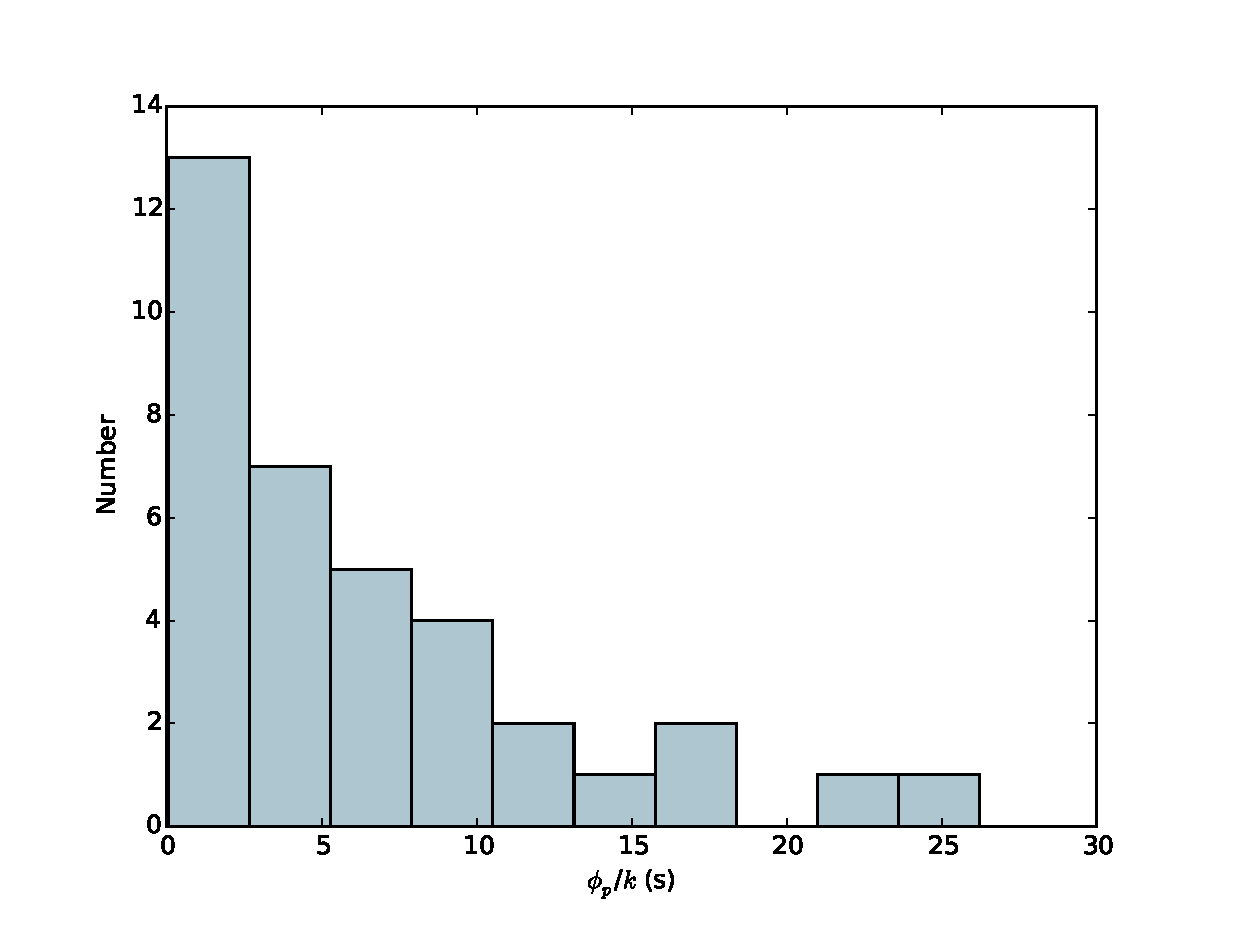
\includegraphics[width=.9\linewidth, trim={0cm 0 0cm 0},clip]{images/appendix_plat_aafluence_n_hist.eps}
  \caption[Histogram showing the distribution of $\phi_p/k$ amongst Normal Bursts.]{A histogram showing the distribution of persistent-emission-normalised plateau fluence $\phi_p/k$ amongst our sample of Normal Bursts.}
  \label{fig:app_hist_phip_n}
\end{figure}

\begin{figure}
  \centering
  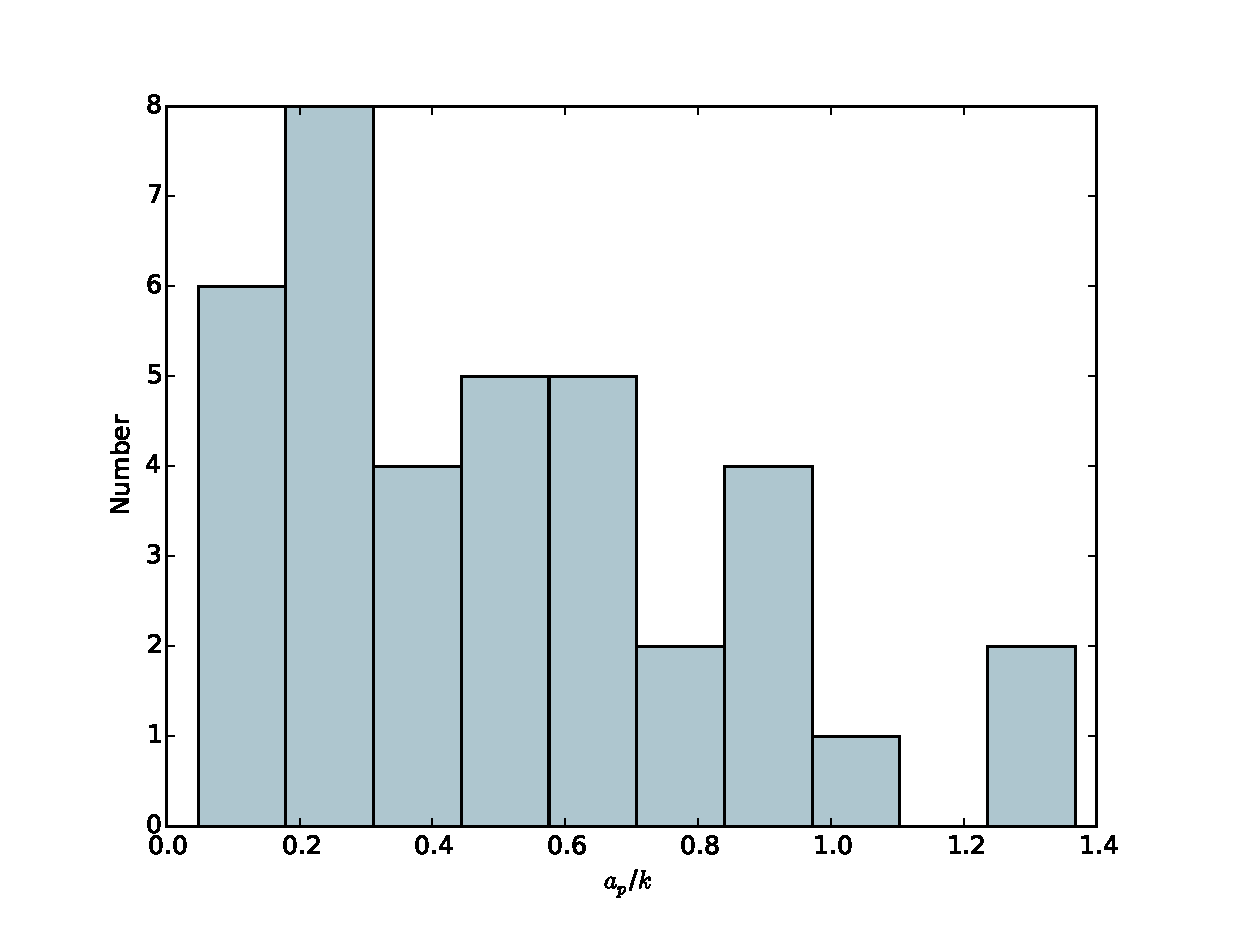
\includegraphics[width=.9\linewidth, trim={0cm 0 0cm 0},clip]{images/appendix_plat_pa_n_hist.eps}
  \caption[Histogram showing the distribution of $a_p/k$ amongst Normal Bursts.]{A histogram showing the distribution of persistent-emission-normalised plateau amplitude $a_p/k$ amongst our sample of Normal Bursts.}
  \label{fig:app_hist_ap_n}
\end{figure}